\documentclass[11pt,a4paper]{article}
\usepackage[margin=2cm,bottom=3cm,foot=1.5cm]{geometry}
\usepackage{graphicx}
\usepackage{amsmath}
\setlength{\parindent}{0pt}
\setlength{\parskip}{0.5ex}
\usepackage{multirow}
\usepackage{braket}
%\usepackage[slovene]{babel}
%\usepackage{dsfont}
\usepackage{mathtools}
\DeclarePairedDelimiter{\evdel}{\langle}{\rangle}
\newcommand{\ev}{\operatorname{E}\evdel}

\title{2. naloga: Klasifikacija zvezdnih spektrov}
\author{Gašper Jalen 28222055}
\date{oktober 2023}

\begin{document}

\maketitle

\section{Uvod}

Pri nalogi smo obravnali spektre zvezd, s pomočjo katerih smo želeli kvalificirati posamezne zvezde in določiti njihoove lastnosti. Osnovni koncept, ki smo ga uporabili je zmanjševanje dimenzij podatkov. Vsak zvezdni spekter namreč vsebuje 2084 točk, torej si ga lahko predstavljamo kot objekt v 2084 dimenzionalnemu prostoru. Naš cilj je zreducirati število dimenzij na npr. dve pri čemer želimo ohraniti kar največ informacije, ki nam jo spekter poda. Poleg večjega seta 10000 spektrov imamo podana še dva manjša seta podatkov, enega s klasificiranimi zvezdami in enega s podanimi fizikalnimi lastnosti zvezd (temperatura, gravitacijski pospešek na površju in kovisnkost). S pomočjo teh dveh setov lahko poizkusimo klasificirati še ostale zvezde in določit njihove lastnosti.

\subsection{PCA}

Sprva za redukcijo dimenzij uporabimo metodo PCA (Principal Component Analysis). Z metodo napravimo dekompozicijo podatkovnega seta v lastne vektorje in lastne vrednosti. Pri tem za željeno natančnost uporabimo željeno število lastnih vektorjev, pri čemer najprej uporabimo tiste z največjo lastno vrednostjo.

Če imamo $n$ spektrov in ima vsak spekter $p$ dimenzij podatki tvorijo matriko $\mathbf{X}$ dimenzij $n \times p$. Podatki so že normirani, tako da jih moramo le še centrirati pri čemer vektor $u_j = 1/n \sum_{i=1}^nX_{ij}$ odštejemo od stolpcov matrike $\mathbf{X}$, da dobimo matriko $\mathbf{B}$

\begin{equation}
	\mathbf{B} = \mathbf{X} - \mathbf{hu}^T,
\end{equation}

kjer je $\mathbf{h}$ vektor enic. Nato izračunamo kovariančno matriko po definiciji

\begin{equation}
	\mathbf{C} = \frac{1}{n-1}\mathbf{B}^*\mathbf{B}
\end{equation}

Na koncu poiščemo še matriko lastnih vektorjev, da velja

\begin{equation}
	\mathbf{V}^{-1}\mathbf{C}\mathbf{V} = \mathbf{D},
\end{equation}

pri čemer si lahko pamaga s SVD razcepom. V matriki $\mathbf{V}$ izberemo poljubno število lastnih vektorjev, ki jih zložimo v matriko $\mathbf{W}$, podatke z reducirnaim številom dimenzij pa dobimo z

\begin{equation}
	\mathbf{T} = \mathbf{D} \cdot \mathbf{W}.
\end{equation}

\subsection{t-SNE}

t-SNE metoda se uporablja za vizualizacijo visokodimenzionalnih podaktov. V našem primeru bo bolj uporabna kot metoda PCA, saj je močno linerna, kot tudi zveze med spektri zvezd in njihovimi fizikalnimi količinami. Same metoda na tem mestu ni matematično opisana, saj je bil cilj naloge spoznavanje z metodo t-SNE in ne njena implementacija.

\section{Podatkovni set}

Pri reševanju naloge sem najprej prikazal nekaj značilnih spektrov, vsaek podane skupine. To sem storil tako, da sem v vsaki naslednji skupini prikazal spekter najbolj različen od prejšnje. V tem primeru sicer ne dobimo 7 spektrov, ki so najbolj različni drug od drugega, a to ni pretirano pomembno. Različnost spektrov sem sicer določil z vsoto kvadrata razlike vseh točk med posameznima spektroma. Značilni spektri so prikazani na sliki \ref{1}.

\begin{figure}[h]
    \centering
    \hbox{\hspace{5em}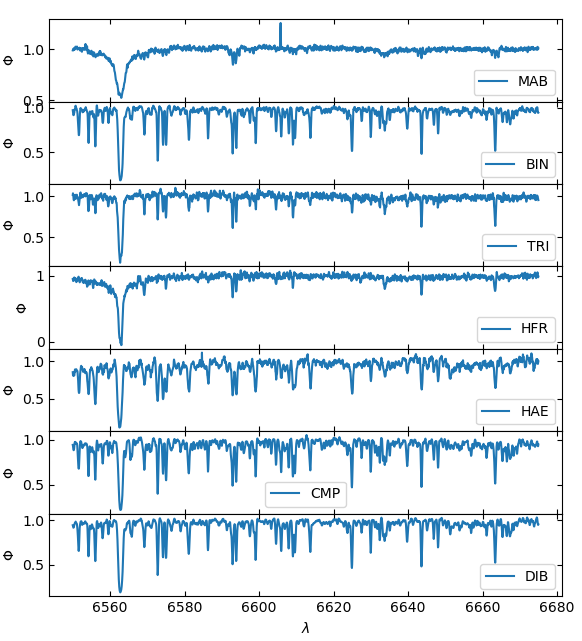
\includegraphics[scale=0.9]{spektri_vizualno}}
    \caption{Primeri spektrov posameznih skupin iz klasificiranega učnega seta.}
    \label{1}
\end{figure}

V značilnosti posameznih skupin iz učnega seta se nisem pretirano poglabljal, oznake skupin pa sem pustil take, kot so bile podane.

\clearpage

\section{Metoda PCA}

Pri metodi PCA prikažemo porazdelitve spektrov po prvih petih komponentah s pomočjo kotnega grafa na sliki \ref{2}.

\begin{figure}[h]
    \centering
    \hbox{\hspace{0em}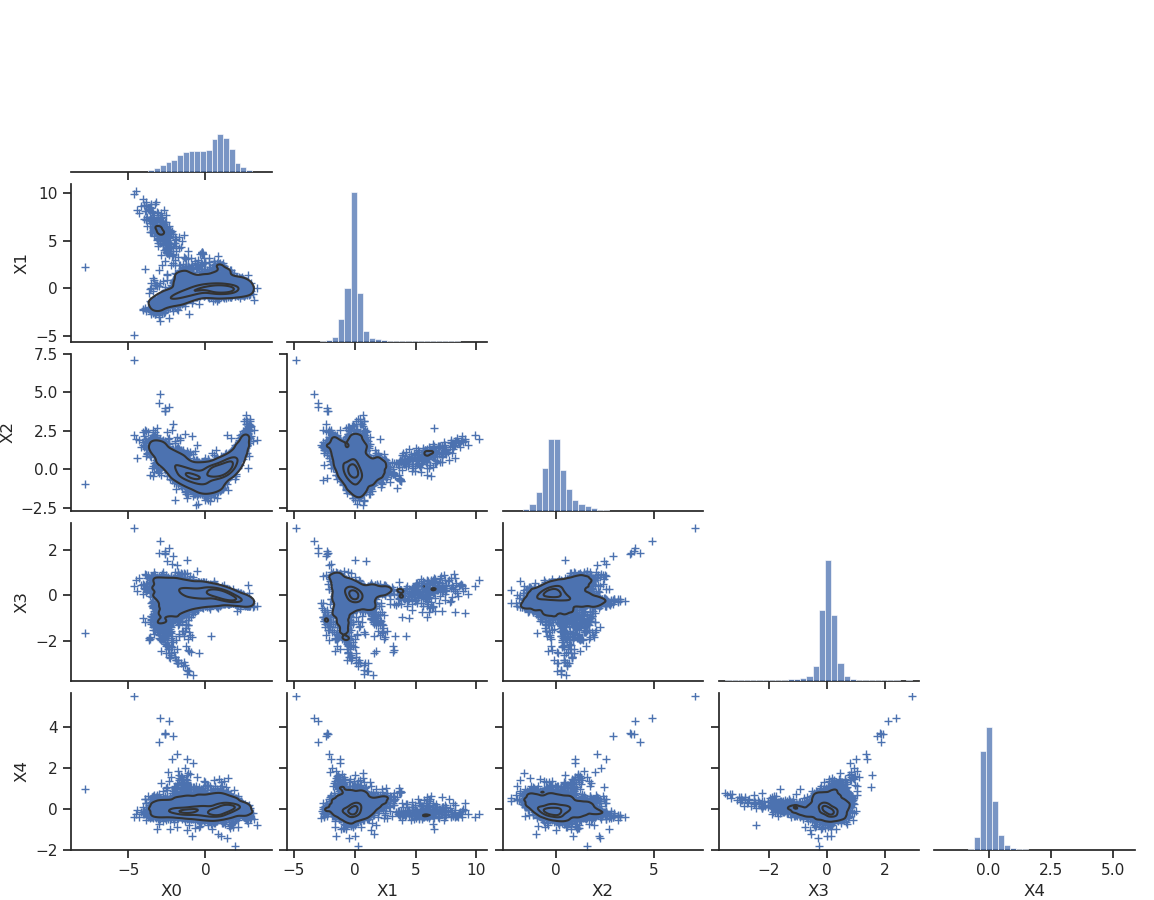
\includegraphics[scale=0.6]{corner_plot}}
    \caption{Porazdelitev spektrov po prvih pet komponentah metode PCA.}
    \label{2}
\end{figure}

Pri tem nas zanima še kako dobro določeno zreducirano število dimenzij opiše originalne podatke, kar definiramo s pomočje normirane energije lastnih vektorjev

\begin{equation}
	g_j^n = \frac{\sum_{k=1}^jD_{kk}}{\sum_{k=1}^pD_{kk}}.
\end{equation}

če torej izberemo za aproksimacijo enako število dimenzij kot na začetku, znaša $g_p^n=1$, kar pomeni da se ne izgubi nič informacije. Normirana energija do $j=10$ je prikazana na sliki \ref{3}. Opazimo, da že za prvih nekaj lastnih vektorjev normirana energija doseže vrednost okoli 0.8 pri čemer začne tudi počasneje naraščati.

\clearpage

\begin{figure}[h]
    \centering
    \hbox{\hspace{9em}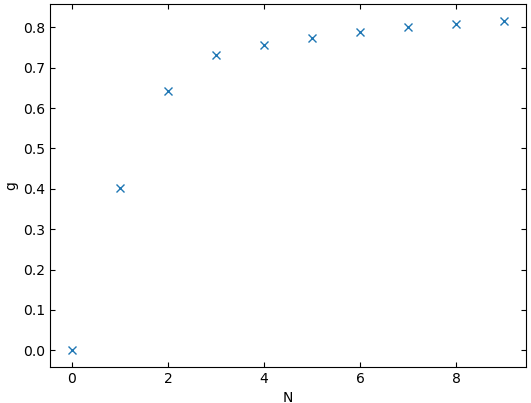
\includegraphics[scale=0.65]{energija}}
    \caption{Porazdelitev spektrov po prvih pet komponentah metode PCA.}
    \label{3}
\end{figure}

Zanima nas kam se pri PCA metodi preslikajo že klasificirane zvezde. Klasifikacija na kotnem grafu za prve tri komponente je prikazana na sliki \ref{4}.

\begin{figure}[h]
    \centering
    \hbox{\hspace{6em}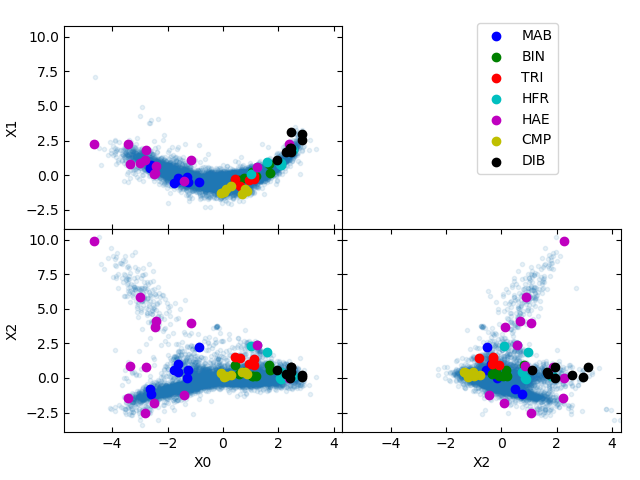
\includegraphics[scale=0.7]{PCA_klasifikacija}}
    \caption{Porazdelitev spektrov po prvih pet komponentah metode PCA.}
    \label{4}
\end{figure}

Klasifikacija na nek način sicer deluje, a je bi na ta način težko določili v katero skupino spada določen spekter. Območja skupin se namreč med seboj prekrivajo, ali pa med njimi ni opaziti jasne meje. Pri tem sta porazdelitvi po prvi in drugi, ter prvi in tretji komponenti približno enako razločni, porazdelitev po drugi in tretji komponenti pa ni več najbolj jasna.

Zanima nas tudi korelacija komponent s posameznimi fizikalnimi količinami, ki je prikazan na sliki \ref{5}. Največjo korelacijo opazimo med prvo komponento in temperaturo, pri čemer temperatura narašča z vrednostjo komponente. Pri temperaturi in ostalih dve komponentah, je sicer še mogoče prepoznati neko značilno smer v katero so podatki bolj razpršeni, prav tako pri korelaciji med $g$ in prvima dvema komponentama, medtem ko za ostale primere skupki točk izgledajo naključni.

\clearpage

\begin{figure}[h]
    \centering
    \hbox{\hspace{7em}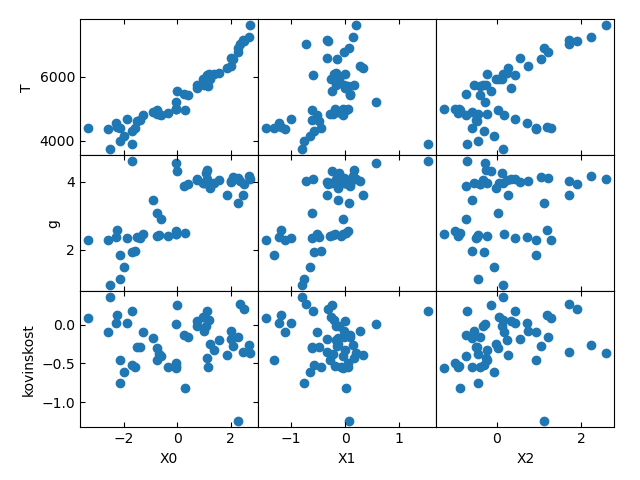
\includegraphics[scale=0.7]{PCA_korelacija}}
    \caption{Korelacija med fizikalnimi količinami in novimi komponentami dobljenimi s PCA metodo. Prikazani so rezultati za prve tri komponente.}
    \label{5}
\end{figure}

\subsection{Kernel PCA}

Dodatno preverimo še delovanje metode kernel PCA, ki za razliko od metode PCA ni popolnoma linearna. Pri metodi sem testiral kako uspešno se ločijo že znani razredi, kar sem prikazal na kotnem grafu za prve tri komponente. Pri tem sta se kot nekoliko bolj uspešni izkazali jedri cosine in poly (polinom pete stopnje), kar je prikazano na slikah \ref{6} in \ref{7}. Pri ostalih jedrih so bili rezultati precej podobni običajni PCA metodi in jih nisem prikazal.

\begin{figure}[h]
    \centering
    \hbox{\hspace{6em}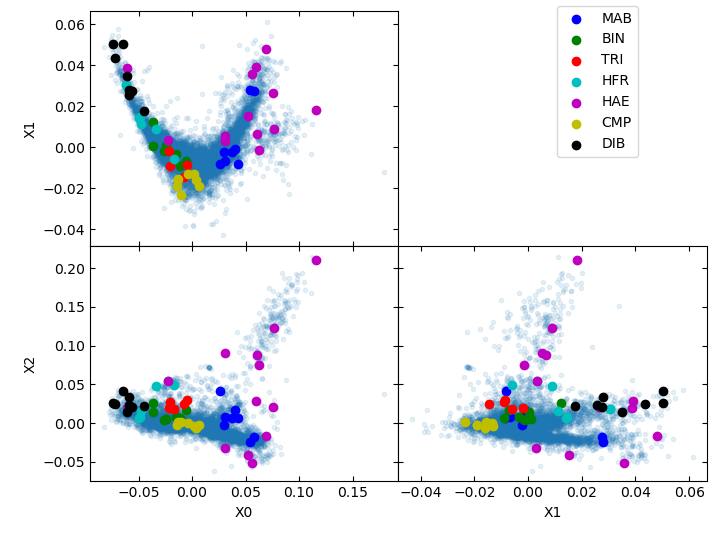
\includegraphics[scale=0.7]{PCA_klasifikacija_cosine}}
    \caption{Porazdelitev spektrov po prvih pet komponentah metode PCA kernel (jedro cosine). Prikazani so rezultati za prve tri komponente.}
    \label{6}
\end{figure}

\begin{figure}[h]
    \centering
    \hbox{\hspace{6em}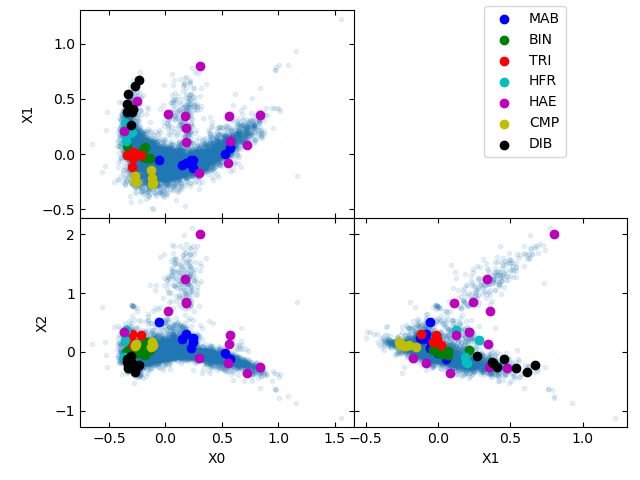
\includegraphics[scale=0.7]{PCA_klasifikacija_poly5}}
    \caption{Porazdelitev spektrov po prvih pet komponentah metode PCA kernel (jedro poly5 - polinom pete stopnje). Prikazani so rezultati za prve tri komponente.}
    \label{7}
\end{figure}

\clearpage

\section{t-SNE}

V drugem delu naloge opravimo redukcijo dimenzij z metodo t-SNE pri čemer obravnavamo le redukcijo na dve dimenziji. Pri tej metodi je potrebno spreminjati parameter perplexity ($p$), ki določa kako metoda grupira posamezne spektre. Rezultati porazdelitve spektrov za različne vrednosti parametra so prikazane na sliki \ref{8}.

\begin{figure}[h]
    \centering
    \hbox{\hspace{2em}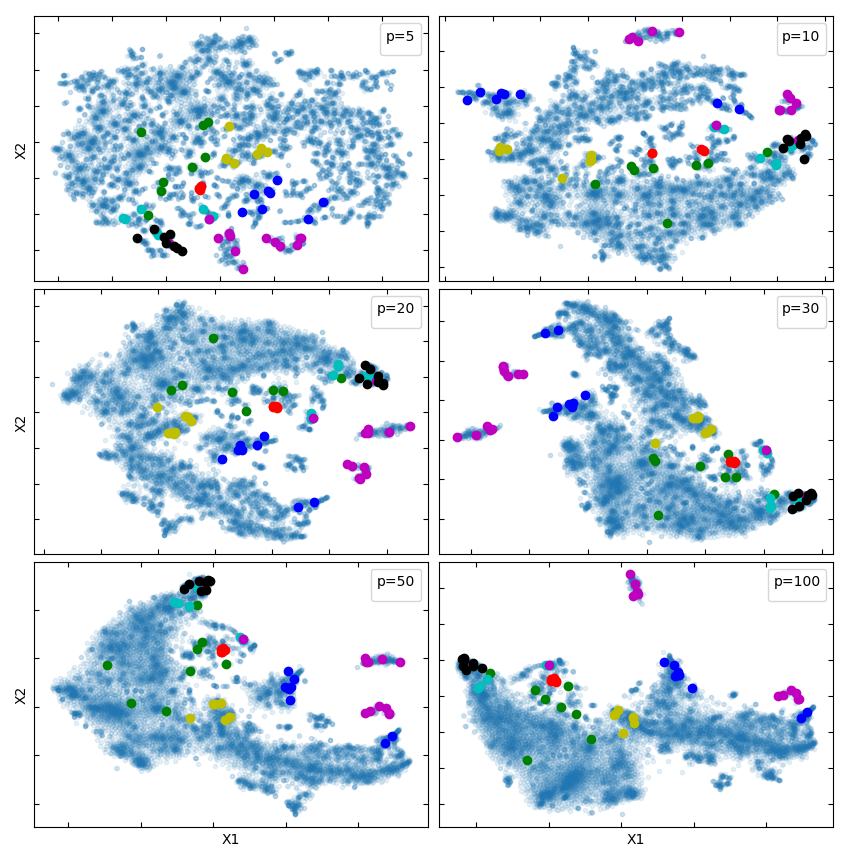
\includegraphics[scale=0.7]{tSNE_klasifikacija}}
    \caption{Porazdelitev spektrov po prvih dveh komponentah metode t-SNE za različne vrednosti parametra $p$. Dodatno so označene že znane skupine zvezd.}
    \label{8}
\end{figure}

Opazimo, da metoda za $p=5$ in $p=10$ spetkrov ne loči najbolje, medtem ko so rezultati za višje vrednosti parametra boljši. Kljub temu pa nobena vrednost posebno ne izstopa po tem da bistveno bolje razloči med posameznimi skupinami, zato sem v nadaljevanju uporabljal parameter $p=20$. Pri tem nekatere skupine zvezd izstopajo precej bolj kot druge. Posebej značilna je skupina HAE (vijolična barva), ki ima v spektru značilno emisijsko črto in 
jo metoda za večino podanih članov skupine jasno loči od ostalih spektrov. Zanimivo se skupina sama pri vseh vrednosti $p$ razdeli na dva otoka.

\clearpage

Poleg klasifikacije nas ponovno zanima korelacija s fizikalnimi količinami. Te so na sliki \ref{9} prikazane z barvo točk na ravnini prvih dveh komponent. Ponovno opazimo največ reda pri temperaturi, kjer ta narašča po polkrožni obliki od zgoraj navzdol. Podoben a manj jasen vzorec opazimo pri pospešku, medtem ko izgleda kovinskost zvezd naključno porazdeljena po obeh koordinatah.

\begin{figure}[h]
    \centering
    \hbox{\hspace{10em}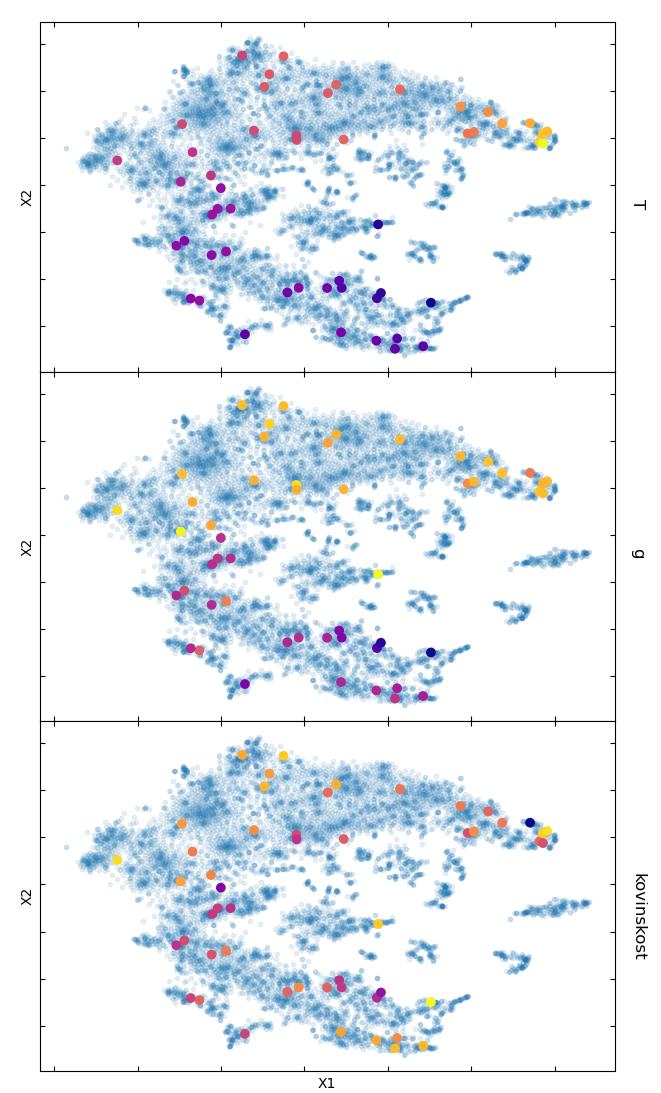
\includegraphics[scale=0.6]{tSNE_corr}}
    \caption{Fizikalne količine zvezd prikazane z barvnimi točkami na porazdelitvi zvezd po prvih dveh komponentah metode t-SNE. Količine so normirane zato skala ni prikazana.}
    \label{9}
\end{figure}

V duhu prejšnje naloge izkoristimo dejstvo, da je temperatura kolerirana z obema koordinatama in poiskusimo s fitom določiti temperaturo vseh zvezd. Za to uporabimo proces GPR z jedrom Matern. Z nekaj prilagajanji parametra $\nu$ (za končni fit je uporabljena vrednost $\nu=2.5$) dobimo podatke o temperaturi za vse spektre, kar je prikazano na sliki \ref{10}.

\clearpage

\begin{figure}[h]
    \centering
    \hbox{\hspace{10em}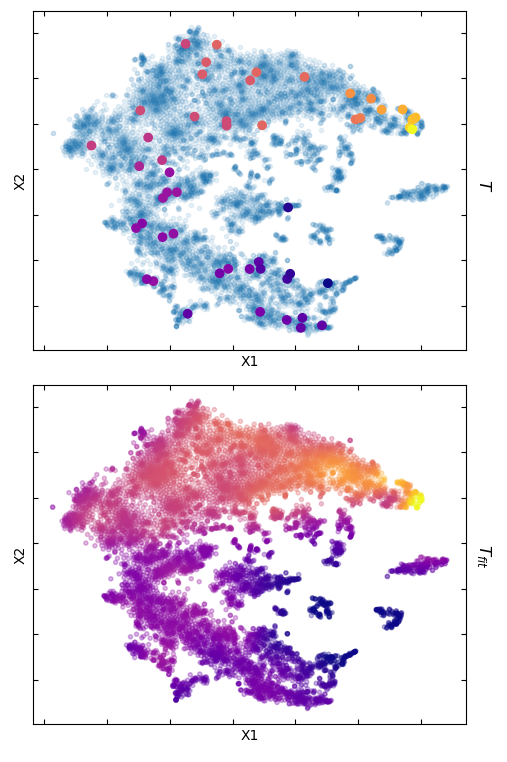
\includegraphics[scale=0.7]{T_fit}}
    \caption{Temperatura zvezd prikazana z barvnimi točkami na porazdelitvi po prvih dveh komponentah metode t-SNE za znane spektre (zgoraj) in za vse spektre (spodaj).}
    \label{10}
\end{figure}

\section{DBSCAN}

Na koncu naloge preizkusimo še avtomatsko klasifikacijo podatko z metodo DBSCAN. Metodi podamo dva parametra in sicer $\varepsilon$, ki vpliva na oddaljenost točk znotraj ene grupe, in minimalno število vzorcev v posamezni grupi (min\_samp). Rezultati klasifikacije za različne vrednosti parametra so prikazani z različnimi barvami na sliki. Za neko smiselno klasifikacijo uporabimo vrednosti $\varepsilon = 1.8$ in $\text{min\_samp}=15$, pri katerih z gručami pokrijemo večino točk, gruče same pa niso pretirano velike.

\clearpage

\begin{figure}[h]
    \centering
    \hbox{\hspace{3em}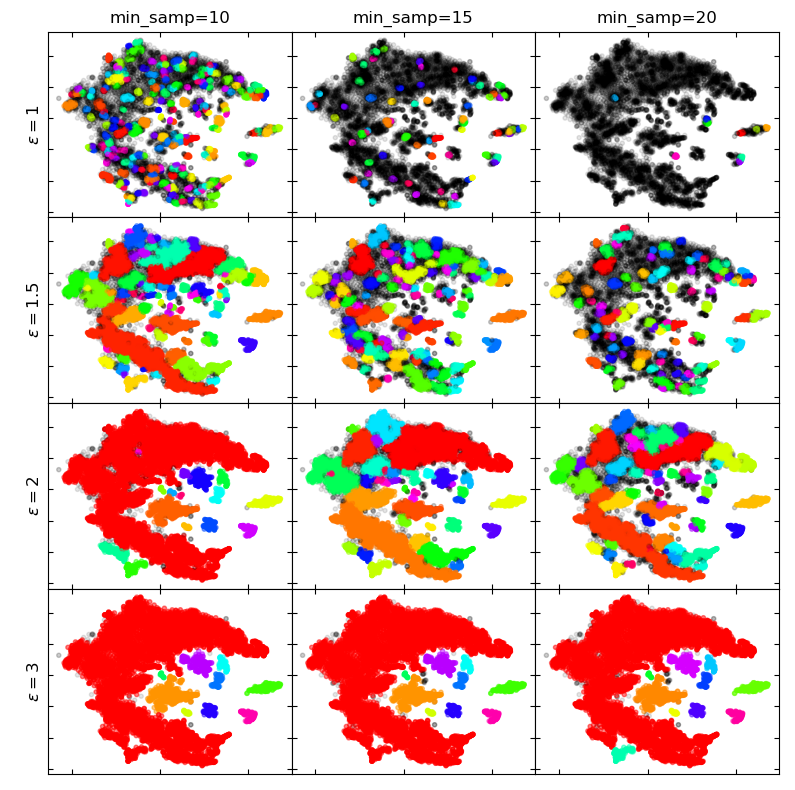
\includegraphics[scale=0.7]{DBSCAN_param}}
    \caption{Klasifikacija točk z metodo DBSCAN za različne parametre $\varepsilon$ in min\_samp. Posamezne gruče so označene z različnimi barvami s črno pa je prikazan šum.}
    \label{10}
\end{figure}

Glede na klasifikacijo z metodo DBSCAN želel v podane skupine v učnem setu razvrstiti še ostale spektre. To sem preprosto storil tako, da sem pogledal v katerih gručah leži največ točk posamezne skupine in vse zvezde iz teh gruč pripisal posamezni skupini. Na tak način sicer večina zvezd ostane neklasificiranih, so pa zato klasificirane zvezde z večjo verjetnostjo pravilno klasificirane. Dodatno sem preveril še eno značilno gručo, ki jo je DBSCAN pri večini parametrov ločil od ostalih in sicer sem jo označil z GA. Na sliki \ref{11} sem prikazal kako spektri iz te gruče odstopajo od nekega tipičnega poveprečnega spektra celotnega seta. Izkaže se da imajo spektri iz tovrstne gruče globlje absorbcijske črte.

Na sliki \ref{12} je prikazana klasifikacija spektrov po skupinah podanih v učnem setu z dodano skupino z globokimi absorbcijskimi črtami. Na podoben način bi verejtno lahko obravnavali vse gruče, ki jih DBSCAN razloči (pri čemer bi si bili določeni spektri med seboj zelo podobni), vendar pa bi zaradi malo znanja o spektrih zvezd na ta način težko prišel do jasnih zaključkov o tipih zvezd. Prav tako mi na tem mestu ni bilo popolnoma jasno ali lahko s klasifikacijo v učnem setu predstavimo vse spektre ali pa del spektrov tvori drugi nepoznane skupine.

\clearpage

\begin{figure}[h]
    \centering
    \hbox{\hspace{6em}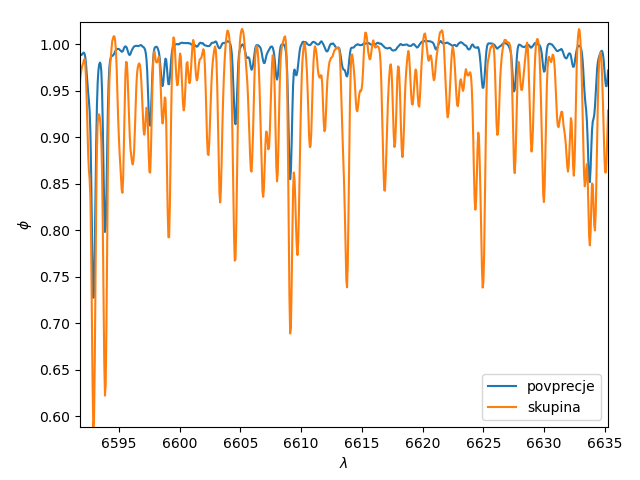
\includegraphics[scale=0.7]{nova_grupa}}
    \caption{Del tipičnega povprečnega spektra in spektra iz izolirane gruče.}
    \label{11}

    \hbox{\hspace{4em}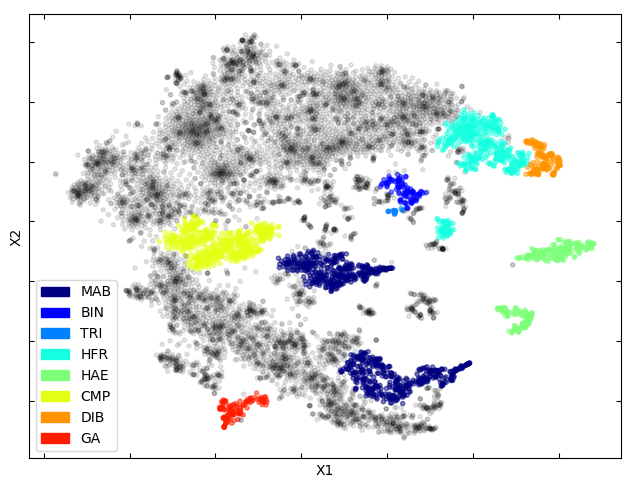
\includegraphics[scale=0.8]{DBSCAN_class}}
    \caption{Klasificarni spektri. Pobarvani so spektri, ki spadajo v skupine iz učnega seta in še spektri, iz skupine GA.}
    \label{12}
\end{figure}

\clearpage

\section{Dodatek}

\begin{figure}[h]
    \centering
    \hbox{\hspace{5em}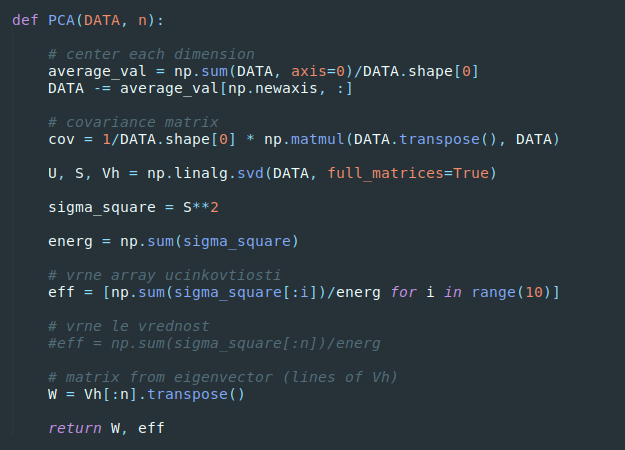
\includegraphics[scale=0.8]{PCA}}
    \caption{Moja implemenacija PCA metode.}
    \label{10}
\end{figure}

\end{document}